\chapter{Experiential Learning\\ of Networking Technologies}
\vskip -15pt

\centerline{{\Huge\sl Understanding TCP Flow Control and Congestion Control}}

\vskip 0.8cm

\begin{center}
{\large\uppercase{Ram P. Rustagi}}, 

\vskip -6pt

Department of CSE, KSIT Bengaluru 


\bigskip
{\large\uppercase{Viraj Kumar,}} 

\vskip -6pt

Divecha Centre for Climate Change, IISc Bengaluru

\end{center}

\vskip 2.3cm



\vfill


%~ \noindent\makebox[\textwidth]{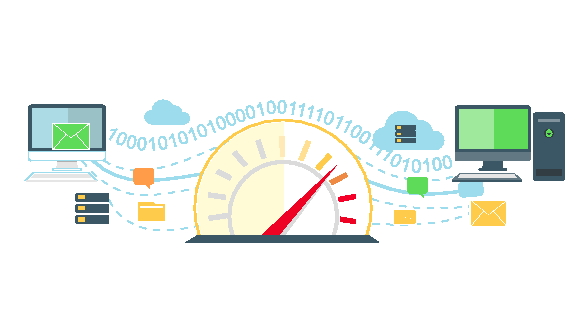
\includegraphics[width=1.05\paperwidth,height=13cm]{src/Figures/chap5.jpg}}
%~ \begin{textblock}{16}(0,8.815)
%~ \noindent\centerimg[width=\paperwidth]{src/Figures/chap5.jpg}
%~ \end{textblock}
\newpage

\begin{multicols}{2}

\section*{Abstract} 

In a TCP connection, the underlying network drops packets when it lacks the capacity to deliver all the packets sent by the sender to the receiver. This phenomenon is called congestion. TCP at the sender’s side will not receive \textit{acks} for these dropped packets. Since TCP is a reliable protocol, the sender must retransmit all these packets. The mechanism used by TCP to deal with such situations is called TCP Congestion Control. In this article, we explain the basics of congestion control and provide experiential exercises to help understand its impact on TCP performance.

\section{Introduction}

We discussed TCP flow control in our previous article \cite{art2-key01}, and we saw that the receiver controls the rate at which the sender can send the data. To achieve this, the receiver informs the sender about its available buffer size (which may be dynamically adjusted), and the sender restricts the transmission of data so that it does not exceed this buffer size. This flow control feature is \textit{independent} of the network capacity – it is \textit{entirely} controlled by the buffer size available at the receiver. If the underlying network’s capacity is greater than the data rate controlled by TCP flow control, then TCP throughput simply depends upon flow control. However, in today’s environment, both the server and client hardware have enough memory available to allow their buffer sizes to be up to 1 GB (the maximum value for flow control supported by TCP). Thus, flow control rarely has an impact on TCP performance, except where memory is a severe constraint e.g., with IoT (Internet of Things) devices in certain instances.

n general, a bigger challenge in attaining high TCP performance is determining the optimal rate at which a server can transmit data to the client. Since TCP \cite{art2-key02] is an end-to-end protocol, this optimal rate is not known at the time when the client connects to the server. Further, this optimal rate can vary significantly – the unpredictable nature of packet arrivals will inevitably place high traffic on certain links at some time, but lower traffic at other times. The mechanism used by the server to discover this optimal transmission rate is called Congestion Control.

Clearly, if the server sends data at a rate lower than the capacity available in the network, it will be under-utilizing the network and it will take longer than necessary to transmit the data. On the other hand, if the server tries to send data at an excessively high rate, the network will choke. More precisely, packets will start to queue at buffers of intermediate network devices. If these buffers become full, any additional packets will be dropped as per the queuing policy (Random Early Detection, Fair Queuing, Weighted Fair Queuing, etc.). At this point, or perhaps even sooner, the sender will fail to receive acknowledgements for packets it had sent (either due to packet drop or timeout), and the sender will be forced to retransmit data packets. These duplicate packets can easily lead to further network delays. Hence, to achieve high performance, it is crucial that the mechanism for Congestion Control adapts rapidly. In reality, this is a complex and challenging task.

\section{Basis of TCP Congestion Control}

Both Flow Control and Congestion Control seek to improve TCP performance. They are inter-related, and they both deal with errors (packets lost/corrupted/discarded) by retransmitting these packets. It is tempting to view these two behaviors as synonymous, but it is important to understand that they are different. At a high level, TCP tries to deliver optimal performance by:
\begin{itemize}
\item[i.] Sending only as much data as can be received by a receiver i.e., data which can be transmitted by the sender without waiting for the \textit{ack}, and should not exceed the receiver’s buffer size. This is dealt with by TCP Flow Control.
\item[ii.] ii. Dynamically adjusting the rate at which the sender transmits data to match the network’s ever-changing capacity. This is dealt with by TCP Congestion Control.
\end{itemize}

It should be intuitively clear that it is essentially impossible to predict the available network capacity ahead of time with reasonable accuracy, given that vast numbers of users are making autonomous decisions that lead to TCP connections and data transfer between clients and servers. In the absence of a good prediction, we use the network capacity in the recent past as the best available estimate of the capacity in the immediate future. Thus, TCP congestion control works by probing the network capacity and adjusting the sender’s transmission rate based upon the probe result. This probing is implicit – there is no explicit probe message. Instead, each data transmission and its \textit{ack} (or even the absence of an \textit{ack}) is used as a probe to estimate network capacity.

In the initial phase of TCP connection and data transfer, early TCP implementations followed a mechanism called \textit{Slow Start}. After a TCP connection is established using a 3-way handshake  \cite{art2-key02], the sender sends one data segment (also known as a congestion window of size 1, or \textit{cwnd} = 1). If it receives the acknowledgement in expected time, it deduces that the network is fine. Then, it repeatedly increases the transmission rate by doubling the congestion window size \textit{cwnd} each time it receives \textit{acks} for all segments within the expected time.

At some point, this exponential growth in transmission rate will exceed the network’s capacity. When some of these segments are lost (or delayed so much that these are considered equivalent to lost), the TCP stack at the receiver will continue to send \textit{acks} for any new data segment it receives out of order. Note such an \textit{ack} will acknowledge only the last segment it received in order, and not the segment it received out of order. This is because TCP is a streaming protocol, so any acknowledgement implies that all the data bytes up to this acknowledgement value have been received. To better understand this point, suppose the sender is sending data in segments of size of 1000 bytes each. The acknowledgement number indicates the offset of the next byte (in the continuous stream of data) that the receiver is expecting in the next data segment. Thus, when receiver receives first 1000-byte segment, the acknowledgement number will be 1001. In general, the acknowledgement for the $N^{th}$ segment will be $1000N + 1$. Now, suppose that the sender has transmitted segments $N–2$, $N–1$, $N$ and $N+1$ and the network loses the \textit{ack} for segment $N–2$ (from receiver to sender after receiving segment $N–2$) and the entire segment $N$ (from sender to receiver). Assume that the network loses no other packets. Thanks to the cumulative acknowledgement\footnote{There are implementations of TCP that follow selective ack rather than cumulative ack, where each packet must  be individually \textit{acked}.} policy followed by TCP, when the sender receives the \textit{ack} for segment $N–1$ (whose acknowledgement number is $1000(N–1) + 1$), it knows that the receiver successfully received segment $N-2$. It can also infer that there may have been some congestion in the network that cause the ack for segment $N–2$ to be dropped, but this seems to have cleared up (since the \textit{ack} for segment $N–1$ was successfully received). After segment $N$ is lost, if the receiver gets segment $N+1$ it will respond with the acknowledgement number $1000(N–1) + 1$ once again, indicating that it is still awaiting the first byte of segment $N$. (The TCP standard RFC 793 \cite{art2-key02} does not specify whether the receiver should discard the segment $N+1$ that was received out-of-order, or store it for future use.) When the sender receives this duplicate \textit{ack}, it can again infer that there is congestion in the network. If the receiver now receives segments $N+2$, $N+3, … $ etc. without receiving segment $N$, the \textit{acks} it responds with for these segments will again have the acknowledgement number $1000(N–1) + 1$. The server can infer that network may have mild congestion, and it can slow down the data transmission rate to avoid aggravating the problem. On the other hand, if the server fails to receive any ack beyond $1000(N–1) + 1$, it can infer that the network is witnessing serious congestion. In this case, the sender will slow the transmission to the lowest possible rate to help network to recover from congestion. TCP has several different implementations, such as TCP Tahoe, TCP Reno, TCP Vegas, etc. which primarily differ in the way they treat congestion. The focus of this article is to understand the core behaviour of TCP, as well as a few other relevant characteristics such as TCP fairness. 

\section{TCP Congestion Management Principles}

The primary mechanism for congestion management adopted by the TCP protocol is to continuously adjust the sender’s transmission rate so as to optimally use the underlying network. Essentially, the sender should try to send data at the highest rate possible without causing congestion in the network. This becomes particularly important when the underlying network’s capacity keeps on changing continuously on account of network usages by other Internet hosts. Further, the only information available to a TCP sender is how many data segments it has sent, which acknowledgements have been received, and the occurrence of timeouts (i.e., failure to receive acknowledgements within expected time). A TCP sender has no knowledge of how many other senders are using the network and what their transmission rates are. TCP makes use of the following criteria to achieve its optimal transmission rate. For a detailed discussion of these criteria, reader should refer to  \cite{art2-key03}.
\begin{itemize}

\item[i.] \textit{Lost segment:} When a segment is lost (when an \textit{ack} is not received within the expected time or when duplicate \textit{acks} are received for earlier segments), it implies some network congestion and thus the sender should decrease its transmission rate.

\item[ii.] \textit{Acknowledgement receipt:} A fresh \textit{ack} (not a duplicate one) for a data segment implies that there is no network congestion at present. A duplicate \textit{ack} implies that the network had some disturbance in the past, but it now seems to have recovered from it – as of now there is no congestion but any increase in traffic might lead to congestion again.

\item[iii.] \textit{Probing of the available bandwidth:} To achieve optimal use of available network bandwidth, TCP follows the strategy of increasing the transmission rate when an ack is received and decreasing the transmission rate when it perceives that its transmitted segment is lost.
\end{itemize}

Using these criteria, Van Jacobson described TCP Congestion Avoidance and Control \cite{art2-key04} in 1998, and further along all the parts of the intertwined congestion control algorithms are summarized in RFC 5681  \cite{art2-key05}.  The TCP Congestion Control algorithm primarily consists of 3 phases, namely
\begin{itemize}

\item[i)] Slow Start phase,

\item[ii)] Congestion Avoidance phase, and

\item[iii)] Fast Recovery phase. 
\end{itemize}

The difference among these various congestion control algorithms are on account of how these 3 phases are intertwined together. We will briefly discuss all these 3 phases and define experiments to imbibe the experiential learning of the same.

TCP is a streaming protocol \cite{art2-key13} and does not honour any message boundary i.e., the receiver never knows how many segments the sender has sent – it only sees a stream of bytes. For simplicity of understanding, we will consider TCP segments in terms of TCP MSS (Max Segment Size)-\cite{art2-key06}\cite{art2-key07}, which on an Ethernet LAN link corresponds to 1460 bytes. Thus, for the description below, segments and acks will be referred to in terms of MSS. Further, the only way TCP can detect packet loss is if the sender times out before receiving an ack. We will refer to this timeout in terms of Round-Trip Time RTT, which correspond to the difference between the time when a sender starts transmitting a segment and the time when it receives its acknowledgement. We also formally define the congestion window (\textit{cwnd}) as the number of TCP segments that can be sent one after the other without waiting for an \textit{ack}. Thus, if there is no congestion in the network, a high value of \textit{cwnd} implies that many segments can be transmitted one after the other, resulting in better throughput for the TCP connection.

When a TCP connection is setup using 3-way handshake, the time duration between SYN sent and SYN-Ack received is used to compute the first RTT. Using this RTT value, and taking into account some variation, an estimated timeout for receiving the \textit{ack} for the next transmitted segment is computed  \cite{art2-key03}. Thus, when the 3-way handshake completes, the sender can estimate the RTT but it does not have any information about the network capacity. Thus, data transmission on this connection starts with \textit{cwnd} conservatively set to 1. When the \textit{ack} for \textit{cwnd}=1 is received within the estimated timeout, \textit{cwnd} is doubled and increased to 2 (the sender transmits 2 segments one followed by the other). When the ack for \textit{cwnd}=2 is received, \textit{cwnd} value is doubled and set to 4, and the sender transmits 4 segments one after the other. This doubling phenomenon is shown in Figure~\ref{chap2-fig01}.

\setcounter{figure}{0}
\begin{figure}[H]
\centering
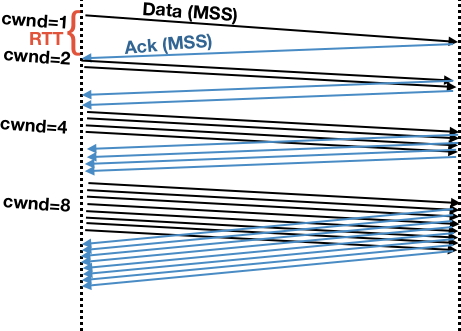
\includegraphics[scale=.95]{src/Figures/chap2/chap2-fig01.jpg}
\caption{TCP Slow start}\label{chap2-fig01}
\end{figure}

Despite the exponential growth in transmission rate, this phase is called Slow start because of the conservative initial value \textit{cwnd}=1. The doubling of \textit{cwnd} can actually be accomplished more efficiently than shown in Figure~\ref{chap2-fig01}. To understand this, suppose \textit{cwnd}=4 i.e., the sender has transmitted 4 segments. One naïve choice would be to wait for all 4 \textit{acks} before doubling \textit{cwnd} to 8. Instead, it is more efficient to increase \textit{cwnd} by 1 each time an \textit{ack} is received: when the first of the 4 \textit{acks} is received \textit{cwnd} becomes 5, when the second \textit{ack} is received \textit{cwnd} becomes 6, etc. When the fourth \textit{ack} is received \textit{cwnd} becomes 8 as shown in Figure~\ref{chap2-fig02}.

\begin{figure}[H]
\centering
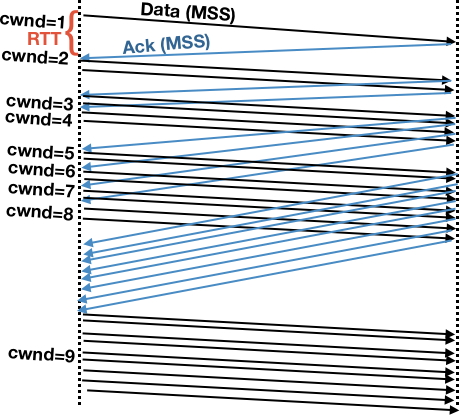
\includegraphics[scale=.95]{src/Figures/chap2/chap2-fig02.jpg}
\caption{Slow Start phase- doubling of cwnd (incrementing it with each ack) and using ssthreshold=8}\label{chap2-fig02}
\end{figure}

It is important to restrict this exponential growth below a limit in order to avoid severe congestion. This limit is called \textit{ssthreshold} (slow start threshold). The setting of the initial value depends upon the TCP stack implementation. For example, \textit{ssthreshold} is 10 for Ubuntu (16.04 LTS). Figure~\ref{chap2-fig03} shows the growth of \textit{cwnd} in slow start phase with initial value of \textit{sshthreshold} as 20. In this figure, the X-axis corresponds to time and the Y-axis corresponds to \textit{cwnd} value. The first round-trip time is about 200ms (actual value: 0.21296s) and \textit{cwnd} starts from value 1 at time T=0s. At time T=0.2s (first RTT), \textit{cwnd} becomes 2. At time T=0.4s (second RTT), \textit{cwnd} becomes 4, and at third RTT (time T=0.66s), \textit{cwnd} becomes 8, and at time T=0.92s (fourth RTT), \textit{cwnd} becomes 16. The exponential growth stops when \textit{cwnd} reaches the slow start threshold (ssthreshold) value of 20 at time 1.08s. 

\begin{figure}[H]
\centering
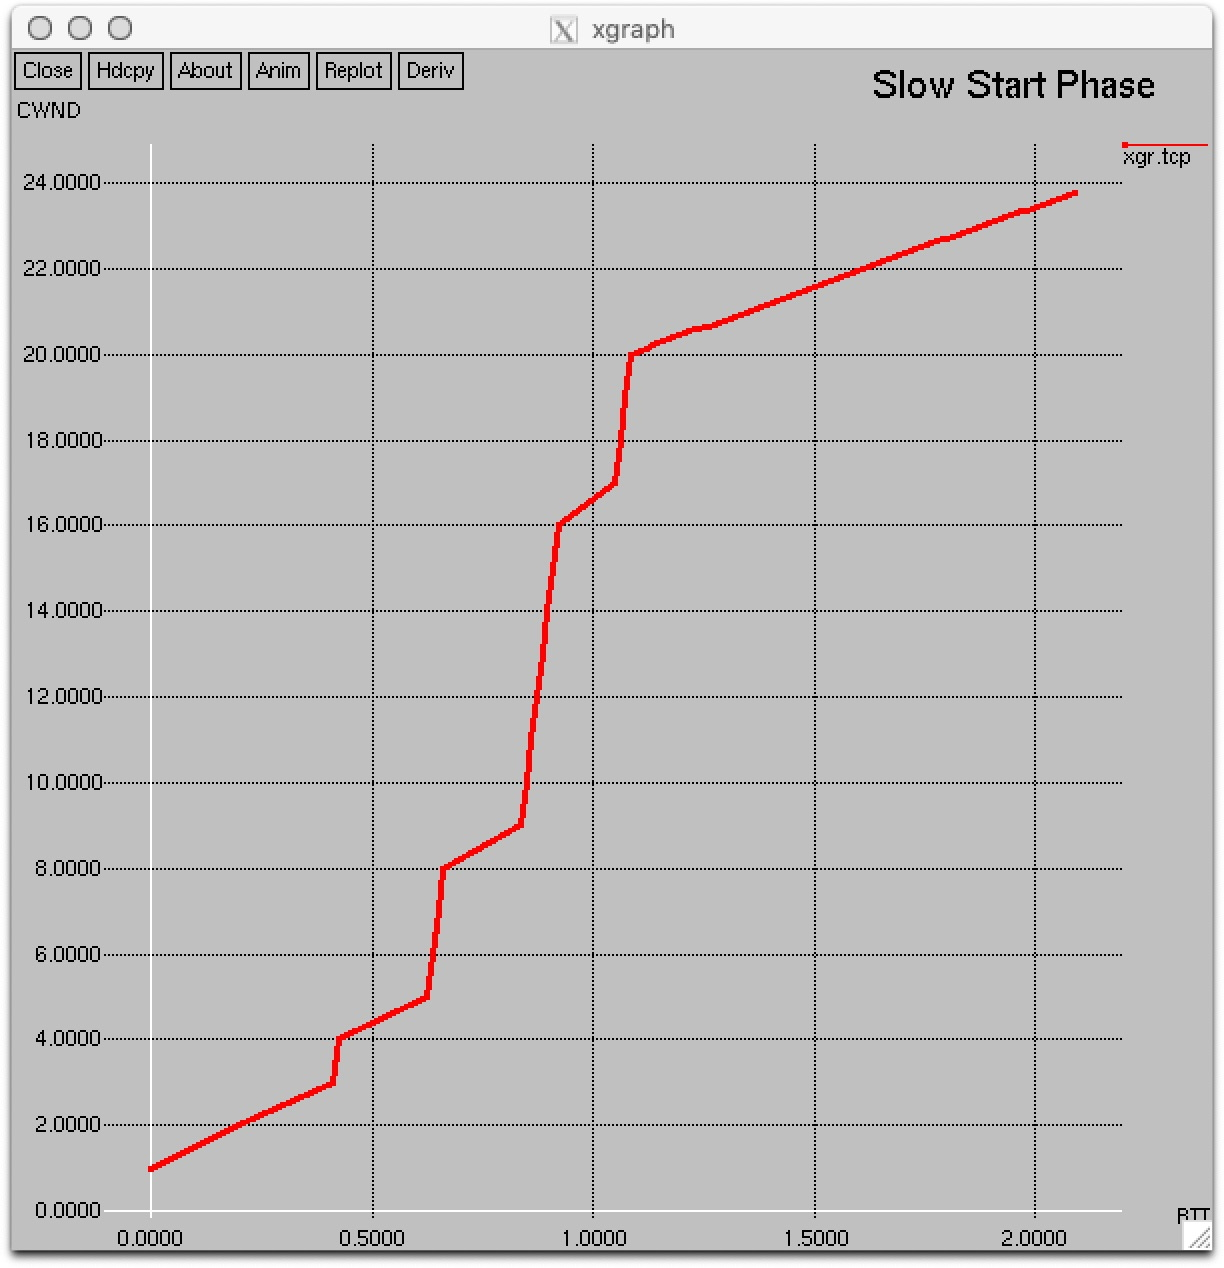
\includegraphics[scale=.95]{src/Figures/chap2/chap2-fig03.jpg}
\caption{Growth of congestion window in Slow Start phase}\label{chap2-fig03}
\end{figure}

The current TCP implementation of operating systems such as Windows, Linux, Mac are optimized, and it may not be easy for the reader to play with TCP tuning parameters to achieve the exact behavior as shown in the graph. The TCP congestion control mechanism followed by Ubuntu Linux is called Cubic \cite{art2-key08} where rather than starting from \textit{cwnd}=1, it simply starts with a higher value depending upon network bandwidth and round-trip time. Thus, to understand the basic TCP slow start phase, an experiment is conducted using NS2 simulator \cite{art2-key09}. Details of installing NS2 and associated tools such as Network Animator (nam) \cite{art2-key10} and Xgraph\cite{art2-key11], are given in the Appendix. To develop a better understanding of the slow start phase experimentally, the reader is requested follow the steps described in Exercise~\ref{chap2-exe01} by configuring desired values of \textit{ssthreshold}, and to plot the graph to study the exponential growth of \textit{cwnd}.

Naturally, an excessively high value of \textit{ssthreshold} can cause congestion and packet loss. Thus, when congestion occurs during the slow start phase (i.e., the sender does not receive acknowledgements for packets it has sent), the sender realizes that network is congested and starts over again with \textit{cwnd}=1.

\section*{Congestion Avoidance phase}

When \textit{cwnd} value reaches \textit{ssthreshold}, it increases the congestion window \textit{cwnd} slowly to avoid possible congestion. In this phase, \textit{cwnd} is increased by 1 when all the previous segments have been acknowledged. This is shown in Figure~\ref{chap2-fig02}  where when \textit{sshthreshold}=8, and after all the acks corresponding to all the 8 transmitted segments are received, \textit{cwnd} is increased by 1 and becomes 9. 

Similarly, in Figure~\ref{chap2-fig03}, \textit{ssthreshold} is set to 20, and thus after \textit{cwnd} becomes 20 at time T=1.08s, it increases linearly with each RTT. The Exercise~\ref{chap2-exe01} described the steps; to experimentally study the linear behaviour of \textit{cwnd} with different value of \textit{ssthreshold} after the former crosses \textit{ssthreshold} value. Thus, at time T=1.35s, \textit{cwnd} becomes 21, and at time T=1.62s, \textit{cwnd} becomes 22 and so on. The general efficient way to increase the \textit{cwnd} is not to wait for all the acks but rather increment the \textit{cwnd} value in such a way that it effectively increases by 1 MSS when all the acks are received. Thus, on each ack received, \textit{cwnd} is increased by \textit{MSS/cwnd} bytes. This is the approach followed in general by any current TCP implementation. The value of \textit{cwnd} will continue to increase linearly till either all the data is transmitted successfully or congestion is encountered When sender detects congestion (deduced, by loss of acknowledgements, it decreases the \textit{cwnd} to mitigate the congestion and thus enters the ${\rm 3}^{rd}$ phase of Fast Recovery. Exercise~\ref{chap2-exe02} describes the experimental set of steps to study the impact of initial value \textit{ssthreshold.}

\section*{Fast Recovery phase}





\section{Basics of TCP Flow Control}

An excellent interactive resource for a basic understanding of flow control is available \cite{art3-key07}. For a more detailed understanding of its implementation using receive window buffer management, let us consider a scenario where the sender needs to transmit 10000 bytes of data. For simplicity, let us assume that the receiver has a buffer of size fixed at 4000 bytes (in reality, this buffer size is dynamically adjusted as per communication needs). Further, let us assume that the sender transmits 1000 bytes every 5 seconds whereas the receiver processes (consumes) 800 bytes every 8 seconds.

The status of the receive window size each time the sender transmits data and the receiver acknowledges the same is shown in Figure~\ref{chap3-fig02}. The following color coding has been used for ease of understanding: Black denotes TCP data transmitted by the sender, blue denotes TCP ack from the receiver, green denotes an update (decrease) in the rwnd (Receive Window) value when data is received from the sender and an ack is sent, and purple denotes an update (increase) in the rwnd value when the receiver application reads the buffer and thus makes some space available. (When rwnd = 4000–$k$, it means that $k$ bytes of data are already filled in the buffer and waiting for the application to read).

The sender first establishes a TCP connection with the receiver by performing a 3-way handshake (first 3 messages in Figure~\ref{chap3-fig02}) \cite{art3-key05}. The receiver informs the sender during the connection setup that its receive buffer size rwnd is 4000 bytes, as shown in Figure~\ref{chap3-fig02}. After the successful connection setup, the sender begins transmitting 1000 bytes of data every 5 seconds: ${\text{T}}_0, {\text{T}}_5, {\text{T}}_{10}, … $ etc. The TCP stack at the receiver sends the ack for each data segment by appropriately updating its rwnd value to indicate the memory available in the receiver’s buffer for this connection. 
\begin{figure}[H]
\centering
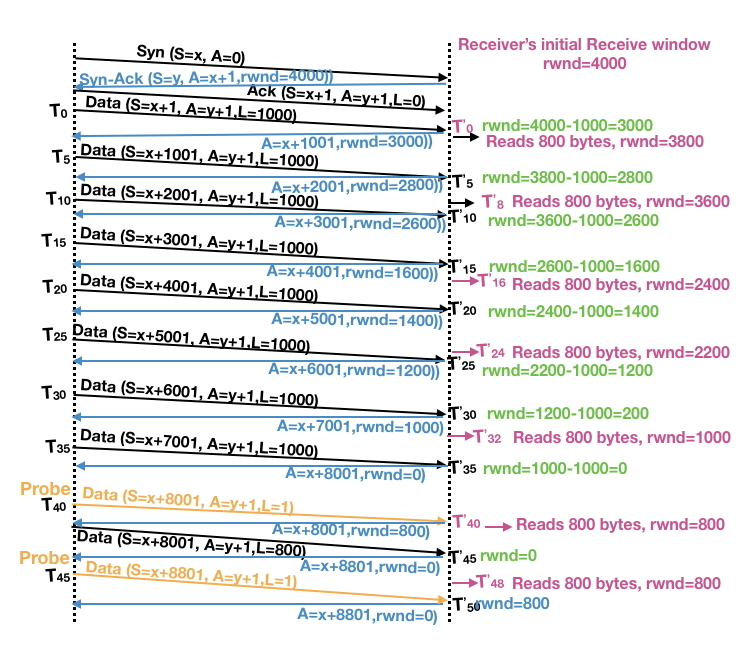
\includegraphics[scale=1.4]{src/Figures/chap3/chap3-fig02.jpg}
\caption{ Adjustment of receive window at receiver}\label{chap3-fig02}
\end{figure}

During the connection setup, the sender is informed that the receiver can receive up to 4000 bytes of data at a time. Thus, at time ${\text{T}}_0$, the sender transmits 1000 bytes as it can transmit up to 4000 bytes. The receiver receives this data at time ${\text{T}}\prime_{\!\!0}$ (slightly after ${\text{T}}_{0}$, because of transmission delay and propagation delay \cite{art3-key08}), stores it in the buffer and updates rwnd to 3000 (4000 - 1000). This updated value is communicated to the sender via the ack. Since the application at the receiver is waiting for data that is now available, it immediately reads 800 bytes from the TCP buffer and starts processing it. This frees 800 bytes from the buffer and hence rwnd is updated to 3800 (3000 + 800). Note that 200 bytes of data are still in the buffer, waiting to be read by the application. At time ${\text{T}}_5$, the sender transmits the next 1000 bytes of data. Once again, the receiver stores this data in the buffer and returns the updated value of rwnd = 2800 (3800-1000) to the sender via the ack. This pattern continues, with the value of rwnd eventually decreasing to 0 after the sender transmits 1000 bytes at ${\text{T}}_{35}$.

\section{Zero Window Probe}

At this point $({\text{T}}_{35})$, the sender cannot transmit any more data since it has received an ack with rwnd=0, indicating that the receiver’s buffer is full. In the scenario we are considering, the application will read 800 bytes from the receiver’s buffer and update rwnd to 800. However, the receiver cannot send a duplicate ack (this can lead to other implications on TCP connections). Thus, both the sender and the receiver appear to be stuck. This deadlocked scenario is generally known as “TCP Zero Window” \cite{art3-key10}\cite{art3-key11}, and it can lead to severe performance issues. Exercise~\ref{chap3-Exe3} describes an experiment to better understand this phenomenon.

Fortunately, TCP provides a mechanism to deal with Zero Window: the sender can periodically transmit a Zero Window Probe (ZWP) message, which could be as small as a single byte of data. Once the receiver gets this TCP message from the sender, it must respond with an ack. Thus, if a ZWP is received after rwnd has been updated to a positive number, the receiver can indicate to the sender that its buffer is no longer full in the ack. Two ZWPs are shown in yellow in Figure~\ref{chap3-fig02}. The first of these probes is initiated at time ${\text{T}}_{40}$. If we assume that the application clears 800 bytes from the reader’s buffer before this probe arrives at time ${\text{T}}\prime_{\!\!40}$, the resulting ack will indicate a positive rwnd value – as shown here. In contrast, consider the second probe initiated at time ${\text{T}}_{45}$. In this case, there still isn’t any free space in the reader’s buffer and hence the ack reports that the value of rwnd is still 0. One or more additional ZWPs (not shown) would have to be issued before data transmission can continue.

ZWPs are used in many other networking applications. For example, consider a network printer that prints documents sent from the machines it is connected to. Since the printer has no data to send, it is the receiver. Suppose that the printer runs out of paper and it takes several minutes to replenish the paper stock. During this interval, the printer may continue to receive documents (without actually printing anything) until its buffer is full. In this case, it will send an ack with the value of rwnd = 0 to the sender machine. This machine can periodically send ZWPs to the printer, and as soon as the paper stock has been replenished, it will resume printing by consuming the data from the receiver buffer. At this point, the value of rwnd will become greater than zero and the ack for subsequent ZWPs will indicate that the printer is ready to receive new documents.

Alert readers may have noticed a potential problem with this seemingly neat mechanism: an adversary can launch a Denial of Service (DoS) attack \cite{art3-key11} by opening connections to a server (sender) and immediately responding with rwnd = 0. This would force the server to waste resources by sending ZWPs (the attacker would respond to each ZWP with rwnd = 0), thus creating a DoS attack. To thwart such attacks, the server follows the standard TCP exponential backoff mechanism where the interval between successive ZWPs doubles each time, up to a pre-configured maximum number of retries. If this limited number of retries is exhausted, the TCP connection may be closed prematurely, releasing resources and avoiding DoS attacks. We now describe a real-life instance where this issue occurred while the first author of this article was managing the cloud deployment of servers.

In this scenario, end users needed to download the roughly 2.5 GB Android image of a mobile phone over a 2 Mbps to 4 Mbps link. In contrast, the servers were\break interconnected via a Gigabit Ethernet network, as shown in Figure~\ref{chap3-fig03}. User connections terminated at the Load Balancer (LB), and the LB would initiate a new connection to the Web Server (WS). The WS, in turn, would connect with the Application Server (AS) and Data Store (DS). Thus, for a single download interaction for end-user $U$, the LB would be dealing with two TCP Connections: a connection ${\text{TCP}}_{U}$ where the LB was the sender and $U$ was the receiver, and a connection ${\text{TCP}}_{WS}$, where the WS was the sender and the LB was the receiver. When the download was initiated, the WS could pump data at a very high rate over ${\text{TCP}}_{WS}$, whereas data was consumed by the user $U$ at a far lower rate over ${\text{TCP}}_{U}$.
\begin{figure}[H]
\centering
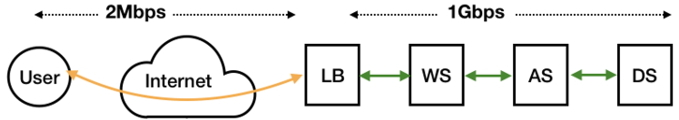
\includegraphics[scale=1.55]{src/Figures/chap3/chap3-fig03.jpg}
\caption{Schematic describing a real-life issue due to TCP Zero Window}\label{chap3-fig03}
\end{figure}

\vskip -.4cm

In order to store as much data as possible from the WS, the LB was forced to rapidly increase its receiver buffer size for ${\text{TCP}}_{WS}$ (by requesting more memory from the OS) until it reached its maximum. This buffer was emptied by copying to the buffer for ${\text{TCP}}_U$, but this occurred at a very slow rate. Due to the huge bandwidth available for ${\text{TCP}}_{WS}$, the WS received an rwnd value of 0 from the LB even after multiple ZWPs. When the retry threshold was exceeded, the connection ${\text{TCP}}_{WS}$ was terminated with about 0.4 GB unsent to the LB. Thus, the end-user was unable to download the entire image.

When this problem was reported in the field, the engineering team responded, as it should by proposing probable causes, based on prior experience and the available data. Suspicion initially fell on the AS application, and when no fault was discovered, the analysis proceeded further. Eventually, and only because of a clear understanding of the TCP Zero Window issue, the problem was diagnosed correctly. (If the first author’s role with the team had not ended shortly after this, the next task would have been to examine strategies for fixing the issue – such as reconfiguring the maximum number of ZWP retries and/or timeout values – and rank these based on the available resources.)

For an experiential understanding of TCP Flow control, reader should follow the steps as defined in Exercise~\ref{chap3-Exe1} and Exercise~\ref{chap3-Exe2}.

\section{Summary}

TCP flow control ensures that the receiver is not overwhelmed by data from the sender. In contrast, the User Datagram Protocol (UDP) does \textit{not} support flow control. Over a UDP connection, the receiver can become overwhelmed and will be forced to drop some of the transmitted data.

Flow control is one of the two key mechanisms that govern TCP performance – the other mechanism is Congestion Control. We will examine Congestion Control in detail in the next article, but briefly it is a mechanism that allows the sender to discover a near-optimal rate at which data can be transmitted over the TCP connection, keeping in mind that network capacity can vary significantly over the course of the data transmission. If the sender transmits data at an excessively low rate, it will be under-utilizing the network capacity and will take more than the optimal time to transmit the entire data. On the other hand, if it sends data at a higher rate than what network can sustain, it will choke the network. As a result, packets will queue up in the network at various stages when buffers become full, some packets will be dropped by intermediate network devices, such as routers, and this will lead to higher queuing delay and wasteful retransmission of packets.

Even though both congestion control and flow control deal with different error conditions, they have the same objective of improving TCP performance and the response of the TCP implementation in both these error conditions is the same – retransmit lost/corrupted/discarded/delayed data segments. Thus, a common misconception is to consider these as equivalent conditions. However, as we shall see in the next article, they are quite different and should be understood differently.

\section{Experiential Exercises}

All the exercise steps described assume that two machines, namely, Client (C\_m) and Server (S\_m) are connected via a network. An example of this connectivity is shown in Figure~\ref{chap3-fig04}. The client machine C\_m is an Ubuntu Linux and server machine could be any machine (Ubuntu/MacOS/Windows) etc. To understand the flow control behavior, two simple Python programs (to be run with python3) are provided: one for the client \url{(accs_client.py)}, which will connect to the server and simply receive data, and the other for the server \url{(accs_server.py)}, which will accept connection from the client and send data. These programs are listed in the Appendix.
\begin{figure}[H]
\centering
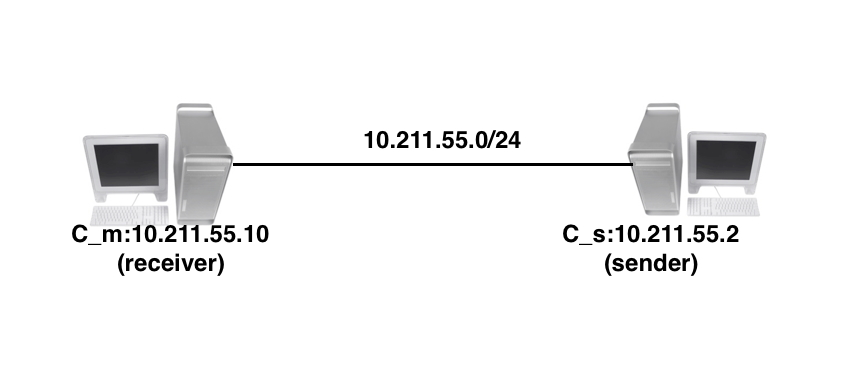
\includegraphics[scale=1.4]{src/Figures/chap3/chap3-fig04.jpg}
\caption{ Basic setup for experiential learning}\label{chap3-fig04}
\end{figure}

\setcounter{section}{0}
\section{Exercise}\label{chap3-Exe1}

\textbf{Topic: Basic understanding of TCP Flow Control with default setup i.e. with Window Scaling}
\begin{itemize}
\item[a.] On the server machine, run the server program as 

\texttt{python3  accs\_server.py -b 200 -d 1 -p 9999}

This will wait for one client to connect and send 200 bytes of data every second.

\item[b.] On the client machine, in one terminal run tcpdump program to look at the window size which is sent. Tcpdump program is used with basic default option and it will show the receive window value (the value of rwnd).  Use the port number 9999 (or any other port of your choice) to capture the traffic. Assuming that the server’s IP address is 10.211.55.2 and uses port number 9999, invoke the command as below

\texttt{sudo tcpdump -n -i enp0s5 host 10.211.55.2 and port 9999}

Please check the Ethernet interface name and replace it appropriately instead of enp0s5.

\item[c.] On the client machine, in another terminal, invoke the client program which will read 100 bytes at a time at an interval of 2 seconds, as below

\texttt{python3 accs\_client.py -s 10.211.55.2 -p 9999 -b 100 -d 2 -c 1000}

Please check the IP address of server and replace it appropriately instead of 10.211.55.2.

\item[d.] The above will connect to the server, and the server will start sending data, which will be displayed on screen.

\item[e.] Look at the output of tcpdump command (in step 2 above), and look at the window size. Note down the value of \texttt{win field} and it is likely to increase with each packet received from server. Given below are sample output for first 4 capture outputs of packets sent from client to server. Notice that \texttt{win field} value starts increasing slowly. The value of ack field is consecutively as 201, 401, 601 etc. i.e. increases by 200 each time indicating that 200 bytes are received. Since data is continuously received, TCP stack slowly increases the client receive buffer size as well.

20:09:21.091424 IP 10.211.55.10.60892 $>$\\
10.211.55.2.9999: Flags [.], ack 201, win 237, options [nop,nop,TS val 1385669 ecr 780230225], length 0

20:09:22.093950 IP 10.211.55.10.60892 $>$\\ 10.211.55.2.9999: Flags [.], ack 401, win 245, options [nop,nop,TS val 1385919 ecr 780231222], length 0

20:09:23.095784 IP 10.211.55.10.60892 $>$\\ 10.211.55.2.9999: Flags [.], ack 601, win 254, options [nop,nop,TS val 1386170 ecr 780232218], length 0

20:09:24.098482 IP 10.211.55.10.60892 $>$\\ 10.211.55.2.9999: Flags [.], ack 801, win 262, options [nop,nop,TS val 1386420 ecr 780233215], length 0

\item[f.] Both the client and server programs are flexible in terms of buffer size (option –b) and delay interval (option –d) and readers are requested to carry the exercise with different values of these options to develop a better understanding of TCP Flow control.
\end{itemize}


\section{Exercise}\label{chap3-Exe2}

\textbf{Topic: TCP Flow Control with Window Scaling disabled.}
\begin{itemize}
\item[a.] On the client machine (Ubuntu), note down the default values (or currently configured) of TCP window scaling and receiver buffer size. Use the following commands to obtain the values.

\texttt{\$ sudo sysctl net.ipv4.tcp\_window\_scaling}

\texttt{ net.ipv4.tcp\_window\_scaling = 1 }
 
 \texttt{\$ sudo sysctl  net.ipv4.tcp\_rmem }
 
 \texttt{net.ipv4.tcp\_rmem = 4096	87380	6291456}
 
 The default value of Window Scaling is 1 implying Window scaling is supported and we will set it to zero to disable the scaling. Similarly, \texttt{\url{net.ipv4.tcp\_rmem}}  provides 3 set of value, first one corresponds to minimum, $2^{\text{nd}}$ one corresponds to default buffer allocation, and last one the max values. Please make a note of these values so as to restore these back after the exercise is completed, otherwise machine may provide poor performance for any TCP connection. For a simple implementation to understand TCP Flow control, set all these values as 4096. Use the following commands to disable the window scaling and receive buffer size. 
 
 \texttt{\$ sudo sysctl-w net.ipv4.tcp\_window\_scaling=0}
 
\texttt{net.ipv4.tcp\_window\_scaling = 0}

\texttt{\$ sudo sysctl -w net.ipv4.tcp\_rmem="4096 4096 4096"}

\texttt{net.ipv4.tcp\_rmem = 4096 4096 4096}

\texttt{\$ sudo sysctl net.ipv4.tcp\_window\_scaling}

\texttt{net.ipv4.tcp\_window\_scaling = 0}

\texttt{\$ sudo sysctl  net.ipv4.tcp\_rmem}

\texttt{net.ipv4.tcp\_rmem = 4096	4096	4096}

These TCP Tuning parameters are set only temporarily and if machine is booted, TCP will start with its default value.

 \item[b.] Repeat the steps of exercise~\ref{chap3-Exe1} i.e. run the server and client program respectively and also observe the value of \texttt{win field} in tcpdump.

\item[c.] As TCP Window scaling is disabled, the rwnd starts from value of 1460 (corresponding to 1500 bytes of Ethernet payload minus 20 bytes of IP header minus 20 bytes of TCP header), and decreases by 200 in each ack packet since data packet contains 200 bytes. A sample dump of tcpdump command for the packets sent from client to server are given below. Thus, the rwnd value starts decreasing from 1460 (initial) to 1260, then 1060, then to 860 and so on. The client program is also reading the data, but at delayed intervals and in smaller amounts, so the read buffer will fill up. You will notice the value remains at 860 for a while (on account of client read as well as some intricate implementations of TCP), and then after a while it starts decreasing again to 660, 460 etc.

21:09:48.598063 IP 10.211.55.10.60904 $>$\\ 10.211.55.2.9999: Flags [.], ack 201, win 1260, options [nop,nop,TS val 1912572 ecr 782330922], length 0

21:09:49.600109 IP 10.211.55.10.60904 $>$\\ 10.211.55.2.9999: Flags [.], ack 401, win 1060, options [nop,nop,TS val 1912823 ecr 782331920], length 0

21:09:50.601628 IP 10.211.55.10.60904 $>$\\ 10.211.55.2.9999: Flags [.], ack 601, win 860, options [nop,nop,TS val 1913073 ecr 782332919], length 0

21:09:51.603529 IP 10.211.55.10.60904 $>$\\ 10.211.55.2.9999: Flags [.], ack 801, win 860, options [nop,nop,TS val 1913323 ecr 782333919], length 0

21:09:52.608485 IP 10.211.55.10.60904 $>$\\ 10.211.55.2.9999: Flags [.], ack 1001, win 860, options [nop,nop,TS val 1913575 ecr 782334920], length 0

21:09:53.610785 IP 10.211.55.10.60904 $>$\\ 10.211.55.2.9999: Flags [.], ack 1201, win 860, options [nop,nop,TS val 1913825 ecr 782335921], length 0

21:09:54.615655 IP 10.211.55.10.60904 $>$\\ 10.211.55.2.9999: Flags [.], ack 1401, win 860, options [nop,nop,TS val 1914076 ecr 782336923], length 0

21:09:55.620261 IP 10.211.55.10.60904 $>$\\ 10.211.55.2.9999: Flags [.], ack 1601, win 660, options [nop,nop,TS val 1914328 ecr 782337926], length 0

21:09:56.622550 IP 10.211.55.10.60904 $>$\\ 10.211.55.2.9999: Flags [.], ack 1801, win 460, options [nop,nop,TS val 1914578 ecr 782338926], length 0
\end{itemize}


\section{Exercise}\label{chap3-Exe3}

\textbf{Topic: TCP Zero Window Probe.}
\begin{itemize}
\item[a.]  Repeat the steps of exercise~\ref{chap3-Exe2} and observe the value of \texttt{win field} for a while. A sample output of TCP exchange between server and client is given below when rwnd becomes zero. This happens after about 12 seconds when 2600 bytes of data have been sent from the server. 

21:19:49.301804 IP 10.211.55.10.60910 $>$\\ 10.211.55.2.9999: Flags [.], ack 1, win 1460, options [nop,nop,TS val 2056798 ecr 782906007], length 0

21:19:49.302448 IP 10.211.55.2.9999 $>$\\ 10.211.55.10.60910: Flags [P.], seq 1:201, ack 1, win 65535, options [nop,nop,TS val 782906007 ecr 2056798], length 200

21:19:49.302484 IP 10.211.55.10.60910 $>$\\ 10.211.55.2.9999: Flags [.], ack 201, win 1260, options [nop,nop,TS val 2056798 ecr 782906007], length 0

:\\
:\\
:

21:20:01.334506 IP 10.211.55.10.60910 $>$\\ 10.211.55.2.9999: Flags [.], ack 2601, win 136, options [nop,nop,TS val 2059806 ecr 782917978], length 0

21:20:07.387763 IP 10.211.55.2.9999 $>$\\ 10.211.55.10.60910: Flags [.], seq 2601:2737, ack 1, win 65535, options [nop,nop,TS val 782923999 ecr 2059806], length 136

21:20:07.387809 IP 10.211.55.10.60910 $>$\\ 10.211.55.2.9999: Flags [.], ack 2737, \underline{\textbf{win 0}}, options [nop,nop,TS val 2061320 ecr 782923999], length 0

21:20:12.494967 IP 10.211.55.2.9999 $>$\\ 10.211.55.10.60910: Flags [.], seq 2737:2738, ack 1, win 65535, options [nop,nop,TS val 782929083 ecr 2061320], \underline{\textbf{length 1}}

21:20:12.495002 IP 10.211.55.10.60910 $>$\\ 10.211.55.2.9999: Flags [.], ack 2737, \underline{\textbf{win 0}}, options [nop,nop,TS val 2062596 ecr 782929083], length 0

21:20:17.900971 IP 10.211.55.2.9999 $>$\\ 10.211.55.10.60910: Flags [.], seq 2737:2738, ack 1, win 65535, options [nop,nop,TS val 782934455 ecr 2062596], \underline{\textbf{length 1}}

21:20:17.901014 IP 10.211.55.10.60910 $>$\\ 10.211.55.2.9999: Flags [.], ack 2737, \underline{\textbf{win 0}}, options [nop,nop,TS val 2063948 ecr 782934455], length 0


\item[b.] In the $6^{\text {th}}$ packet in above display (in actual there will be few more packets which have not been shown here for brevity), from client to server, the value of win field is 0 (shown as underlined and in bold) implying that receiver buffer has become full.

\item[c.] In the subsequent packet ($7^{\text {th}}$), which is from server to client, it is a probe packet as can be determined from length value of 1 (shown in bold and underline).

\item[d.] In response to Zero Window Probe, client still responds with win=0 ($8^{\text{th}}$ packet) as its receive buffer is still full. 

The above explains the phenomenon of Zero Window Probe. Please restore the value of TCP window scaling and memory allocation for receive buffer to its system default value by using the following command (or even performing a reboot).

\texttt{\$ sudo sysctl -w net.ipv4.tcp\_window\_scaling=1}

\texttt{\$ net.ipv4.tcp\_window\_scaling = 0}

\texttt{\$ sudo sysctl -w net.ipv4.tcp\_rmem=" 4096 87380 6291456"}

\texttt{net.ipv4.tcp\_rmem = 4096 87380 6291456}
\end{itemize}

\section*{Appendix}
{\lstset{xleftmargin=1cm}
{\bf Client program: accs\_client.py.}\\
{\bf \#--------------------------------------------------------------------------------}
\begin{lstlisting}[language=Caml,basicstyle=\small]
#!/usr/bin/python3
import socket
import time
import argparse

parser = argparse.ArgumentParser
	(description=
	 "Simple Server for N/w Delays")
parser.add_argument('-s', '--server', 
		type=str, required=True)
parser.add_argument('-p', '--port', 
		type=int, default=9999)
parser.add_argument('-c', '--count', 
		type=int, default=10)
parser.add_argument('-d', '--delay', 
		type=int, default=5)
parser.add_argument('-b', '--buffer', 
		type=int, default=50)
args = parser.parse_args()

ip_addr = args.server
port = args.port
count = args.count
delay = args.delay
buffer = args.buffer

srvr_addr = (ip_addr, port)
sock = socket.socket(socket.AF_INET, 
		socket.SOCK_STREAM)
sock.connect(srvr_addr)

for i in range(1,count):
    data = sock.recv(buffer)
    print ("received:", data)
    time.sleep(delay)

sock.close()
\end{lstlisting}}
{\bf \#--------------------------------------------------------------------------------}

\bigskip

{\bf Server program: accs\_server.py.}\\
{\bf \#--------------------------------------------------------------------------------}

\begin{lstlisting}[language=Caml,basicstyle=\small]
#!/usr/bin/python3
import socket
import time
import argparse

parser = argparse.ArgumentParser
	(description=
	 "Simple Server for N/w Delays")
parser.add_argument('-s', '--server', 
		type=str, default="0.0.0.0")
parser.add_argument('-p', '--port', 
		type=int, default=9999)
parser.add_argument('-d', '--delay',  
		type=int, default=1)
parser.add_argument('-b', '--buffer',  
		type=int, default=100)
args = parser.parse_args()

ip_addr = args.server
port = args.port
delay = args.delay
buffer = args.buffer

sock = socket.socket(socket.AF_INET, 
		socket.SOCK_STREAM)
srvr_addr = (ip_addr, port)
sock.bind(srvr_addr)
sock.listen(5)
connsock, client = sock.accept()
print("received a conn from", str(client))

while True:
    msg = "A" * buffer
    print ("Sending:", msg)
    sent = connsock.send(msg.encode('ascii'))
    time.sleep(delay)
\end{lstlisting}
{\bf \#--------------------------------------------------------------------------------}\hfill \raisebox{-.1cm}{\includegraphics[scale=.9]{src/Figures/circledC.eps}}

\begin{thebibliography}{99}
\bibitem{art3-key01}RFC 793, “Transmission Control Protocol “, Information Sciences Institute, USC, CA, Sep 1981,

 \url{https://tools.ietf.org/html/rfc793.} Last accessed May 2019.

\bibitem{art3-key02}  RFC 1323, “TCP extensions for Long Delay Paths “, Jacobson, Braden, Oct 1988 

\url{https://tools.ietf.org/html/rfc1072}, Last accessed May 2019.

\bibitem{art3-key03} RFC 7323, “TCP extensions for High Performance“, Borman, Braden, Jacobson, Scheffenegger, Oct 1988 

\url{https://tools.ietf.org/html/rfc7323#page-8}, Last accessed May 2019.

\bibitem{art3-key04} Ram Rustagi, Viraj Kumar, “Understanding Transport Layer Basics”, ACCS journal of Computing and Communications, Vol 2, Issue 3, Sep 2018. 

\url{https://acc.digital/experiential-learning-of-networking-technologies-understanding-transport-layer-basics/}, last accessed Nov 2018.

\bibitem{art3-key05}Ram Rustagi, Viraj Kumar, “Understanding TCP States- Part I”, ACCS journal of Computing and Communications, Vol 2, Issue 4, Dec 2018 

\url{https://acc.digital/experiential-learning-of-networking-technologies-understanding-tcp-states-part-1/}, last accessed May 2019

\bibitem{art3-key06}Ram Rustagi, Viraj Kumar, “Understanding TCP States- Part I”, ACCS journal of Computing and Communications, Vol 3, Issue 1, Mar 2019

 \url{https://acc.digital/experiential-learning-of-networking-technologies-understanding-tcp-states-part-2/}, last accessed June 2019

\bibitem{art3-key07} Understanding TCP Flow control with interactive animations,

 \url{https://media.pearsoncmg.com/aw/ecs_kurose_compnetwork_7/cw/content/interactiveanimations/flow-control/index.html}, last accessed May 2019.

\bibitem{art3-key08} Ram Rustagi, Viraj Kumar, “Understanding Network Delays”, ACCS journal of Computing and Communications, Vol 1, Issue 3, Dec 2017;  

\url{https://acc.digital/experiential-learning-of-networking-technologies-understanding-network-delays/}, last accessed Nov 2018.

\bibitem{art3-key09} Kurose, Ross, “Computer Networking: A Top Down Approach”, section 3.5.5, $6^{\text{th}}$ edition, Pearson, 

\bibitem{art3-key10}RFC 1122, “Requirements for Internet Hosts -- Communication Layer”, Braden, IETF, Oct 1989. 

\url{https://tools.ietf.org/html/rfc1122}, Last accessed June 2019.

\bibitem{art3-key11} RFC 6429, “TCP Sender Clarification for Persist Conditions”, Bashyam, Jethanandani, Ramaiah, Dec 2011, 

\url{https://tools.ietf.org/html/rfc6429}, last accessed June 2019.

\end{thebibliography}
\end{multicols}



\noindent
\begin{tabular}{V{2.5}cp{14.2cm}V{2.5}}
\clineB{1-2}{2.5}
 &\\
\raisebox{-4cm}{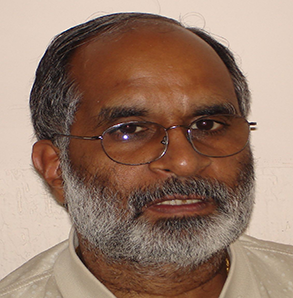
\includegraphics{src/Figures/authors/Rustagi_RPR-PP-Photo.png}} & 

\centerline{\large\bf Prof. Ram P. Rustagi}

\bigskip
Dr.~Ram P. Rustagi is currently working as Professor, CSE dept, KSIT Bangalore, and honed up his academic skills with Ph.D from IIT Delhi, and M.Tech from IISc Bangalore. Prior to KSIT, at Cavisson Systems, he mentored new technology development using Machine Learning techniques in Security and Performance Monitoring. At PES University, he had taught Undergraduates, Post Graduates students, and successfully guided 3 Ph.D scholars. At PESU, he brought innovations in teaching computer network and security courses, and introduced practical experiential learning exercises.\\
&\\  
\raisebox{-3.7cm}{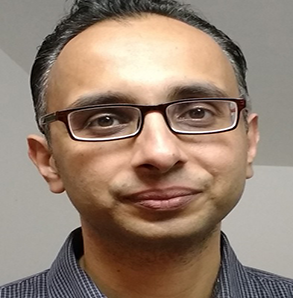
\includegraphics{src/Figures/authors/Viraj_Kumar.png}} & 

\centerline{\large\bf Prof. Viraj Kumar}

\bigskip
Dr.~Viraj Kumar is a Visiting Professor at the Divecha Centre for Climate Change, IISc Bangalore and the Vice-Chair of ACM India’s Special Interest Group in Computer Science Education (iSIGCSE). He was a consultant to the Committee to draft the National Education Policy (2017-18), and contributed to two education-related task groups of the Karnataka Knowledge Commission (2014-16). He holds a PhD in Computer Science from the University of Illinois at Urbana-Champaign.\\
&\\
\clineB{1-2}{2.5}
\end{tabular}

\vskip 1cm

\begin{figure}[H]
\centering

\includegraphics[scale=.15]{src/Figures/QR-codes/qr-code_experiential-learning.png}

\medskip

{\large\sf Access this article on the Web}
\end{figure}


















